\documentclass[12pt , a4paper]{article}
\usepackage[spanish]{babel}
\usepackage[utf8]{inputenc}
\usepackage{graphicx}
\graphicspath{ {./images/} }



\title{Práctica MARP\\Algorítmo de dijkstra con montículo sesgado}
\author{Juan Chozas Sumbera}

\begin{document}
	
	\maketitle
	\begin{center}
		
\includegraphics[width=\textwidth]{logo_UCM.jpg}
	\end{center}
	
	\newpage
	
\section{Implementación}
	
	He elegido Java como lenguaje para variar, ya que el año pasado hice las dos prácticas en C++. Para representar grafos he elegido listas de adyacencia: una lista de pares de enteros para cada vértice (vértice adyacente, coste de la arista).
	
	El montículo sesgado contiene un entero (tamaño) y un nodo (raíz). La inclusión de la operación \textit{decrecerClave} trae la necesidad de almacenar y mantener la tabla (clave: entero, valor: nodo) que almacena todos los nodos del montículo. Un nodo contiene un puntero a su nodo padre, además de a sus dos hijos. Para una implementación eficiente de \textit{decrecerClave}, uso estos punteros para \textit{cortar} el nodo objetivo del padre y unirlo con el montículo restante.
	
\section{Ejecución}
	Incluyo también un script llamado \texttt{dijkstra} que puede usarse para compilar y ejecutar el programa. Admite varios argumentos, de los cuales solo es obligatorio \texttt{-n NUM}, usado para generar un grafo de \texttt{NUM} nodos. Se puede omitir este argumento en caso de usar la opción \texttt{-t 1} o \texttt{-t 2}, que ordena la ejecución de uno de los casos de prueba. Los grafos usados para probar el algoritmo se crearon de forma aleatoria, y se puede elegir la semilla con la opción \texttt{-s SEM}. La opción \texttt{-h} proporciona más información acerca de las opciones.
	

\section{Medición}
\subsection{Métodos empleados}
	El grafo se genera de antemano, y el vértice inicial siempre es el 0. Los tiempos se han medido usando la función \texttt{System.nanoTime()} midiéndose únicamente el tiempo transcurrido durante la ejecución del algoritmo de la siguiente forma:
	\begin{verbatim}
	long t1 = System.nanoTime();
	resultados = dijkstra(g, 0);
	long t2 = System.nanoTime();
	\end{verbatim}
	
	La máquina usada durante la medición siempre estaba enchufada a la corriente. El sistema operativo que usa es Ubuntu 18.04, y todas las ejecuciones se realizaron en terminales \texttt{tty}. Desactivé la conexión de la máquina a Internet con las instrucciones \texttt{ip link set wlp2s0 down} y \texttt{service network-manager stop}. Las ejecuciones se hicieron usando los siguientes instrucciones:
	\begin{verbatim}
	for i in `seq 5 5 100`; do 
	    ./dijkstra -n $i -a -d -i 6 > tiempos/$i; 
	done
	for i in `seq 125 25 1000`; do 
	   ./dijkstra -n $i -a -d -i 6 > tiempos/$i;
	do ne
	for i in `seq 1050 50 5000`; do 
	    ./dijkstra -n $i -a -d -i 6 > tiempos/$i; 
	done
	\end{verbatim}
	A partir de 5000 nodos, saltaban excepciones relacionadas al límite de memoria. Las opciones indican
	\begin{itemize}
		\item el número de nodos (\texttt{-n \$i})
		\item que se imprima el número de aristas generadas (\texttt{-a})
		\item que el grafo generado sea dirigido (\texttt{-d})
		\item que se ejecute el algoritmo 6 veces (\texttt{-i 6})
	\end{itemize} 
	La última opción resulta en 6 medidas distintas, de las cuales la primera siempre tenía un valor mucho más elevado al resto (al menos en grafos con no muchos vértices). En la siguiente sección aparecen gráficas que descartan esta primera medida en el cálculo de la media, y otras que la incluyen. También hay gráficas de grafos no dirigidos para los mismos rangos de vértices (mismas instrucciones pero sin la opción \texttt{-d}).
	
	Finalmente, procesé las medidas en la carpeta \texttt{tiempos} con dos scripts, \texttt{averages.sh} y \texttt{edges.sh}, con el fin de calcular las medias de las medidas y obtener el numero de aristas generadas para la prueba, respectivamente.


\section{Resultados}

	A continuación aparecen las gráficas. Las dos primeras no tienen en cuenta la primera ejecución. El valor del primero tiempo leído era mucho mayor que el del resto, que no variaba mucho de uno a otro. Esto lo pude comprobar observando el comportamiento en un número alto de iteraciones con la opción \texttt{-i}. No veo una explicación a esto, por lo tanto las dos primeras gráficas omiten el resultado.
	
	\hspace*{-.15\linewidth}
	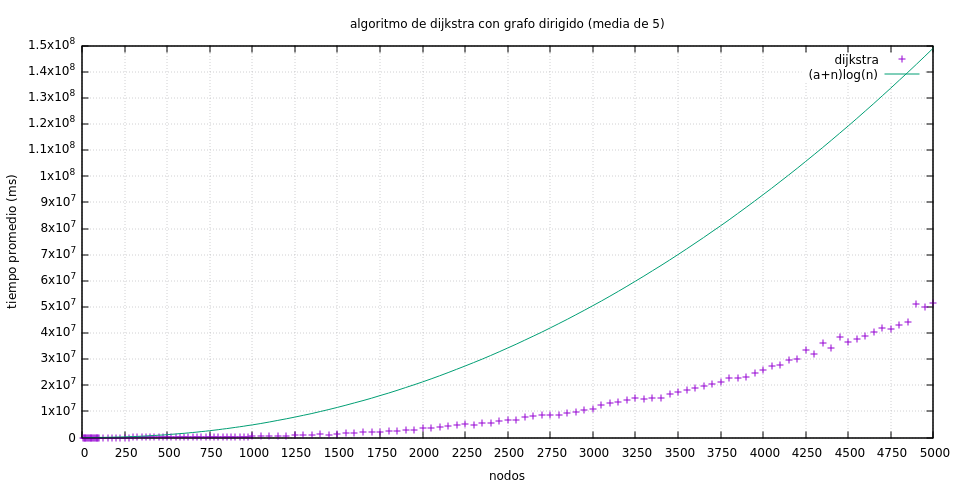
\includegraphics[width=1.25\hsize]{dir5.png}
	\texttt{Gráfica 1 - Grafos dirigidos sin tener en cuenta la primera medida}
	La curva del tiempo es menos acentuada que la de la cota superior, pero la curva tiene la misma forma. Estimo que la curva de las medidas está en \texttt{z*(a+n)log(n)}, con \texttt{z} entre 0.3 y 0.5. Puede ser porque el algoritmo termina sin visitar todos los vértices: con grafos dirigidos es más probable que haya nodos inaccesibles por haber restricciones de dirección en las aristas. 
	
	
	\newpage
	\hspace*{-.15\linewidth}
	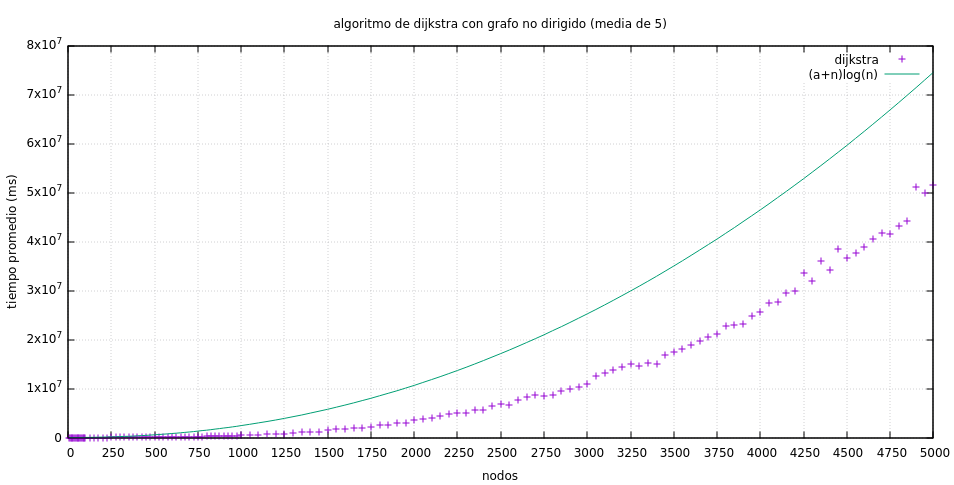
\includegraphics[width=1.25\hsize]{nodir5.png}
	\texttt{Gráfica 2 - Grafos no dirigidos sin tener en cuenta la primera medida}
	La curva de las medidas se asemeja más la curva de la cota superior que cuando los grafos son dirigidos. Estas medidas también parecen seguir la curva de la cota superior: diría que la curva es \texttt{z*(a+n)log(n)}, con \texttt{z} entre 0.5 y 0.7.  Yo creo que esto se debe al hecho de que hay más aristas que en un grafo dirigido, lo cual hace más probable que todos los nodos sean alcanzables. Es menos probable que el algoritmo termine sin haber visitado todos los nodos.


	\newpage
	\hspace*{-.15\linewidth}
	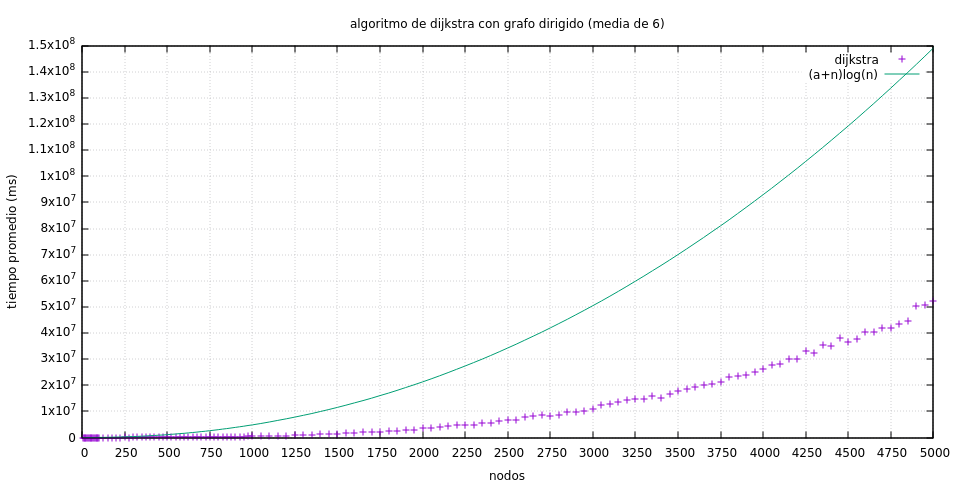
\includegraphics[width=1.25\hsize]{dir6.png}
	\texttt{Gráfica 3 - Grafos dirigidos teniendo en cuenta la primera medida}
	Es muy similar a la gráfica 1. Algunos puntos suben y otros bajan, pero la diferencia es apenas notable.
	
	
	\newpage
	\hspace*{-.15\linewidth}
	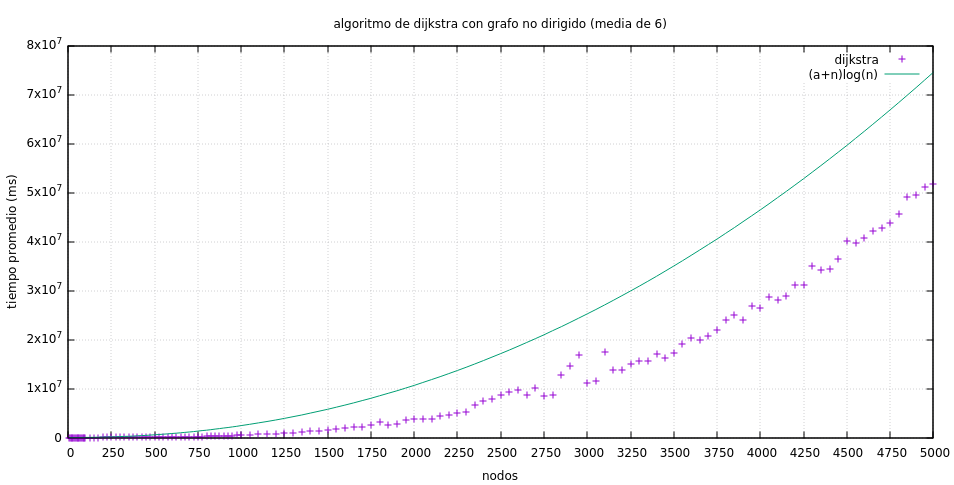
\includegraphics[width=1.25\hsize]{nodir6.png}
	\texttt{Gráfica 4 - Grafos no dirigidos teniendo en cuenta la primera medida}
	La inclusión de la primera medida es más notable en esta gráfica que en la 3: entre 2650 y 3000 nodos hay mucha más varianza que en la gráfica 2. Creo que se le puede echar la culpa a la máquina en este subconjunto de pruebas, pues todos los tiempos son mayores. Fuera de este pequeño rango, las medidas no son muy diferentes a las de la gráfica 2.
	Comparando con la segunda gráfica, puedo concluir que para cada primera ejecución en el rango de nodos mencionado, el tiempo de medido es mucho más elevado al de las otras 5 ejecuciones. No sabría explicar por qué solo pasa en la primera ejecución, ni por qué hay tanta diferencia en este rango de nodos.

\end{document}